% ===========================================================================
%  TikuOS — TikuKits DS: Linked List for Embedded Systems
%  Beamer Presentation
% ===========================================================================
\documentclass[aspectratio=169, 10pt]{beamer}

% ---- Theme ----------------------------------------------------------------
\usetheme{Madrid}
\usecolortheme{whale}
\setbeamertemplate{navigation symbols}{}
\setbeamertemplate{footline}{%
  \leavevmode\hbox{%
    \begin{beamercolorbox}[wd=.33\paperwidth,ht=2.5ex,dp=1ex,center]{author in head/foot}%
      \usebeamerfont{author in head/foot}\insertshortauthor
    \end{beamercolorbox}%
    \begin{beamercolorbox}[wd=.34\paperwidth,ht=2.5ex,dp=1ex,center]{title in head/foot}%
      \usebeamerfont{title in head/foot}\insertshorttitle
    \end{beamercolorbox}%
    \begin{beamercolorbox}[wd=.33\paperwidth,ht=2.5ex,dp=1ex,right]{date in head/foot}%
      \usebeamerfont{date in head/foot}\insertshortdate{}\hspace*{2em}%
      \insertframenumber{}/\inserttotalframenumber\hspace*{2ex}
    \end{beamercolorbox}}%
  \vskip0pt%
}

% ---- Packages -------------------------------------------------------------
\usepackage{listings}
\usepackage{graphicx}
\usepackage{hyperref}
\usepackage{booktabs}
\usepackage{multirow}
\usepackage{tikz}
\usetikzlibrary{arrows.meta, positioning, shapes.geometric, calc,
                decorations.pathreplacing, fit}
\usepackage{amsmath}

% ---- Code listing style ---------------------------------------------------
\lstset{
  basicstyle=\ttfamily\scriptsize,
  keywordstyle=\color{blue}\bfseries,
  commentstyle=\color{gray},
  stringstyle=\color{red!70!black},
  showstringspaces=false,
  breaklines=true,
  frame=single,
  rulecolor=\color{black!30},
  backgroundcolor=\color{blue!3},
  tabsize=4,
}
\lstdefinestyle{cstyle}{
  language=C,
  morekeywords={uint8_t,uint16_t,uint32_t,int32_t,
                tiku_kits_ds_elem_t,
                TIKU_KITS_DS_OK,TIKU_KITS_DS_ERR_NULL,
                TIKU_KITS_DS_ERR_FULL,TIKU_KITS_DS_ERR_EMPTY,
                TIKU_KITS_DS_ERR_PARAM,TIKU_KITS_DS_ERR_BOUNDS,
                TIKU_KITS_DS_ERR_NOTFOUND,
                TIKU_KITS_DS_LIST_MAX_NODES,
                TIKU_KITS_DS_LIST_NONE,
                NULL},
}

% ---- Metadata -------------------------------------------------------------
\title[TikuKits DS]{TikuKits DS: Linked List for Embedded Systems}
\subtitle{Simple. Ubiquitous. Intelligence, Everywhere.}
\author[Ambuj Varshney]{Ambuj Varshney \\ \texttt{ambuj@tiku-os.org}}
\date{\today}

% ===========================================================================
\begin{document}

% ---------------------------------------------------------------------------
\begin{frame}
\titlepage
\end{frame}

% ---------------------------------------------------------------------------
\begin{frame}{Outline}
\tableofcontents
\end{frame}

% ===========================================================================
\section{Motivation}
% ===========================================================================

\begin{frame}{Why a Linked List on MCUs?}
\begin{columns}[T]
\begin{column}{0.48\textwidth}
\begin{block}{Embedded Use Cases}
\begin{itemize}
  \item \textbf{Timer lists} --- ordered list of pending timers
  \item \textbf{Task queues} --- dynamic insertion/removal of processes
  \item \textbf{Sensor registry} --- register/unregister sensors at runtime
  \item \textbf{Event chains} --- linked list of pending event handlers
\end{itemize}
\end{block}

\begin{block}{The Problem}
\begin{itemize}
  \item Standard linked lists use \texttt{malloc}/\texttt{free}
  \item MCUs have no heap or very limited heap
  \item Pointer-based nodes waste memory on 32-bit addresses
  \item Need dynamic insertion/removal without arrays shifting
\end{itemize}
\end{block}
\end{column}

\begin{column}{0.48\textwidth}
\begin{center}
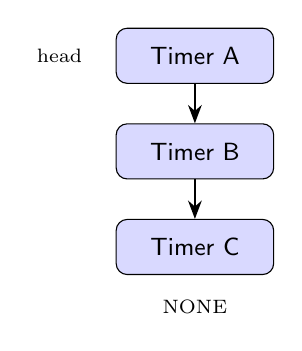
\begin{tikzpicture}[
    >=Stealth, node distance=0.5cm,
    nodebox/.style={draw, rounded corners, minimum height=0.7cm,
        minimum width=2cm, font=\small\sffamily}
  ]
  \node[nodebox, fill=blue!15] (n0) {Timer A};
  \node[nodebox, fill=blue!15, below=0.5cm of n0] (n1) {Timer B};
  \node[nodebox, fill=blue!15, below=0.5cm of n1] (n2) {Timer C};
  \node[font=\scriptsize, left=0.3cm of n0] {head};
  \draw[->, thick] (n0) -- (n1);
  \draw[->, thick] (n1) -- (n2);
  \node[font=\scriptsize, below=0.2cm of n2] {NONE};
\end{tikzpicture}
\end{center}

\vspace{0.5em}
\begin{alertblock}{Our Solution}
\textbf{Pool-allocated} singly linked list. Static array of nodes,
\texttt{uint8\_t} indices instead of pointers, free list for allocation.
No heap required.
\end{alertblock}
\end{column}
\end{columns}
\end{frame}

% ===========================================================================
\section{Architecture}
% ===========================================================================

\begin{frame}{The Pool Allocator Pattern}
\begin{columns}[T]
\begin{column}{0.55\textwidth}
\textbf{Key innovation:} Replace \texttt{malloc}/\texttt{free} with a
\textbf{static pool} of pre-allocated nodes.

\vspace{0.5em}
\textbf{Two linked lists share the same array:}
\begin{enumerate}
  \item \textbf{Active list} --- nodes in use (user data)
  \item \textbf{Free list} --- available nodes for allocation
\end{enumerate}

\vspace{0.5em}
\textbf{Allocate:} Pop a node from the free list head.\\
\textbf{Deallocate:} Push the node back onto the free list head.

\vspace{0.5em}
\textbf{Index-based:} Node references are \texttt{uint8\_t} indices
(0--254) instead of pointers. On a 16-bit MCU, this saves 1 byte per
link. On 32-bit MCUs, it saves 3 bytes per link.

\vspace{0.3em}
\texttt{TIKU\_KITS\_DS\_LIST\_NONE = 0xFF} serves as the
sentinel (end-of-list marker).
\end{column}

\begin{column}{0.42\textwidth}
\begin{center}
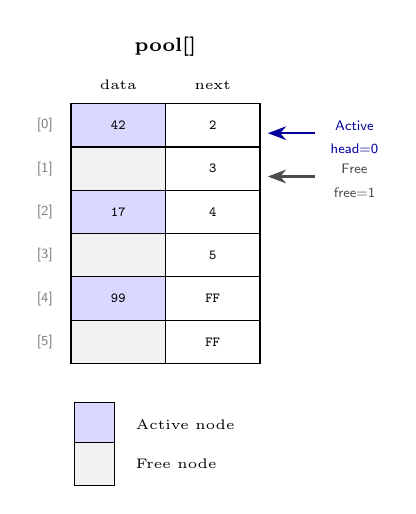
\begin{tikzpicture}[
    >=Stealth,
    cell/.style={draw, minimum width=1.2cm, minimum height=0.55cm,
                 font=\tiny\ttfamily},
    idx/.style={font=\tiny\sffamily, text=gray}
  ]
  % Pool array
  \node[font=\scriptsize\bfseries] at (0.6, 1.0) {pool[]};

  \foreach \i/\d/\n/\c in {
    0/42/2/blue!15,
    1/{}/3/gray!10,
    2/17/4/blue!15,
    3/{}/5/gray!10,
    4/99/FF/blue!15,
    5/{}/FF/gray!10} {
    \node[cell, fill=\c] (p\i) at (0, -\i*0.55) {\d};
    \node[cell] (pn\i) at (1.2, -\i*0.55) {\n};
    \node[idx, left=0.1cm of p\i] {[\i]};
  }

  \node[font=\tiny, above=0.05cm of p0] {data};
  \node[font=\tiny, above=0.05cm of pn0] {next};

  % Active list arrow
  \node[font=\tiny\sffamily, text=blue!60!black] at (3.0, 0.0) {Active};
  \draw[->, blue!60!black, thick] (2.5, -0.1) -- (1.9, -0.1);
  \node[font=\tiny\sffamily, text=blue!60!black] at (3.0, -0.3)
    {head=0};

  % Free list arrow
  \node[font=\tiny\sffamily, text=gray!60!black] at (3.0, -0.55) {Free};
  \draw[->, gray!60!black, thick] (2.5, -0.65) -- (1.9, -0.65);
  \node[font=\tiny\sffamily, text=gray!60!black] at (3.0, -0.85)
    {free=1};

  % Legend
  \node[cell, fill=blue!15, minimum width=0.5cm] at (-0.3, -3.8) {};
  \node[font=\tiny, right=0.1cm] at (0.0, -3.8) {Active node};
  \node[cell, fill=gray!10, minimum width=0.5cm] at (-0.3, -4.3) {};
  \node[font=\tiny, right=0.1cm] at (0.0, -4.3) {Free node};
\end{tikzpicture}
\end{center}
\end{column}
\end{columns}
\end{frame}

% ===========================================================================
\section{Data Structure}
% ===========================================================================

\begin{frame}[fragile]{The \texttt{tiku\_kits\_ds\_list} Structures}
\begin{columns}[T]
\begin{column}{0.48\textwidth}
\begin{lstlisting}[style=cstyle,
  title={ds/list/tiku\_kits\_ds\_list.h}]
#define TIKU_KITS_DS_LIST_MAX_NODES 16
#define TIKU_KITS_DS_LIST_NONE 0xFF

struct tiku_kits_ds_list_node {
    tiku_kits_ds_elem_t data;
    uint8_t next; /* index or NONE */
};

struct tiku_kits_ds_list {
    struct tiku_kits_ds_list_node
        pool[TIKU_KITS_DS_LIST_MAX_NODES];
    uint8_t  head;     /* first active  */
    uint8_t  free;     /* first free    */
    uint16_t count;    /* active nodes  */
    uint16_t capacity; /* runtime cap   */
};
\end{lstlisting}
\end{column}

\begin{column}{0.48\textwidth}
\textbf{Memory footprint} (default config):\\
Per node: $4 + 1 = 5$ bytes\\
Total: $16 \times 5 + 1 + 1 + 2 + 2 = 86$ bytes\\
All statically allocated --- no heap.

\vspace{0.5em}
\begin{block}{Why \texttt{uint8\_t} Indices?}
\begin{itemize}
  \item Pointer on MSP430 = 2 bytes
  \item Pointer on ARM Cortex-M = 4 bytes
  \item \texttt{uint8\_t} index = 1 byte everywhere
  \item Supports up to 255 nodes (0xFF = sentinel)
\end{itemize}
\end{block}

\vspace{0.3em}
\begin{alertblock}{Sentinel Value}
\texttt{LIST\_NONE = 0xFF} marks end-of-list for both
the active chain and the free chain.
\end{alertblock}
\end{column}
\end{columns}
\end{frame}

% ===========================================================================
\section{API Reference}
% ===========================================================================

\begin{frame}[fragile]{Complete API}
\begin{table}
\centering
\small
\begin{tabular}{@{}lp{7.5cm}@{}}
\toprule
\textbf{Function} & \textbf{Description} \\
\midrule
\texttt{tiku\_kits\_ds\_list\_init(list, cap)}
  & Initialize pool with \texttt{cap} nodes, build free list \\
\midrule
\texttt{tiku\_kits\_ds\_list\_push\_front(list, val)}
  & Insert at head --- $O(1)$ \\
\texttt{tiku\_kits\_ds\_list\_push\_back(list, val)}
  & Append at tail --- $O(n)$ \\
\texttt{tiku\_kits\_ds\_list\_insert\_after(list, idx, val)}
  & Insert after node at pool index \texttt{idx} \\
\midrule
\texttt{tiku\_kits\_ds\_list\_pop\_front(list, \&val)}
  & Remove and return head element --- $O(1)$ \\
\texttt{tiku\_kits\_ds\_list\_remove(list, idx)}
  & Remove node at pool index --- $O(n)$ predecessor search \\
\midrule
\texttt{tiku\_kits\_ds\_list\_find(list, val, \&idx)}
  & Linear search, returns pool index of first match \\
\texttt{tiku\_kits\_ds\_list\_get(list, idx, \&val)}
  & Read data at a pool index \\
\midrule
\texttt{tiku\_kits\_ds\_list\_clear(list)}
  & Return all nodes to free pool \\
\texttt{tiku\_kits\_ds\_list\_size(list)}
  & Current active node count \\
\texttt{tiku\_kits\_ds\_list\_head(list)}
  & Pool index of head node \\
\texttt{tiku\_kits\_ds\_list\_next(list, idx)}
  & Pool index of next node after \texttt{idx} \\
\bottomrule
\end{tabular}
\end{table}
\end{frame}

% ===========================================================================
\section{Configuration}
% ===========================================================================

\begin{frame}[fragile]{Compile-Time Configuration}
\begin{columns}[T]
\begin{column}{0.48\textwidth}
\begin{lstlisting}[style=cstyle,
  title={Configurable parameters}]
/* Maximum pool size */
#ifndef TIKU_KITS_DS_LIST_MAX_NODES
#define TIKU_KITS_DS_LIST_MAX_NODES 16
#endif

/* Sentinel: end of list */
#define TIKU_KITS_DS_LIST_NONE 0xFF
\end{lstlisting}

\vspace{0.3em}
\begin{block}{Element Type}
Defined in \texttt{tiku\_kits\_ds.h}:
\begin{lstlisting}[style=cstyle]
#ifndef TIKU_KITS_DS_ELEM_TYPE
#define TIKU_KITS_DS_ELEM_TYPE int32_t
#endif
typedef TIKU_KITS_DS_ELEM_TYPE
    tiku_kits_ds_elem_t;
\end{lstlisting}
Override at compile time:
\texttt{-DTIKU\_KITS\_DS\_ELEM\_TYPE=int16\_t}
\end{block}
\end{column}

\begin{column}{0.48\textwidth}
\begin{lstlisting}[style=cstyle,
  title={Runtime initialization}]
struct tiku_kits_ds_list lst;

/* Use 8 of the 16 available nodes */
tiku_kits_ds_list_init(&lst, 8);

/* Or use maximum capacity */
tiku_kits_ds_list_init(&lst,
    TIKU_KITS_DS_LIST_MAX_NODES);
\end{lstlisting}

\vspace{0.3em}
\begin{table}
\centering
\scriptsize
\begin{tabular}{@{}rrr@{}}
\toprule
\textbf{Max Nodes} & \textbf{Elem Size} & \textbf{RAM (bytes)} \\
\midrule
8  & 4 (int32)  & 46 \\
16 & 4 (int32)  & 86 \\
16 & 2 (int16)  & 54 \\
32 & 4 (int32)  & 166 \\
\bottomrule
\end{tabular}
\end{table}
\end{column}
\end{columns}
\end{frame}

% ===========================================================================
\section{Pool Allocator Details}
% ===========================================================================

\begin{frame}[fragile]{Pool Allocator: Alloc and Free}
\begin{columns}[T]
\begin{column}{0.48\textwidth}
\begin{lstlisting}[style=cstyle,
  title={pool\_alloc --- pop from free list}]
static uint8_t pool_alloc(
    struct tiku_kits_ds_list *list)
{
    uint8_t idx;

    if (list->free ==
            TIKU_KITS_DS_LIST_NONE) {
        return TIKU_KITS_DS_LIST_NONE;
    }

    idx = list->free;
    list->free = list->pool[idx].next;
    list->pool[idx].next =
        TIKU_KITS_DS_LIST_NONE;
    return idx;
}
\end{lstlisting}

Pop the head of the free chain.\\
$O(1)$ --- no searching required.
\end{column}

\begin{column}{0.48\textwidth}
\begin{lstlisting}[style=cstyle,
  title={pool\_free --- push to free list}]
static void pool_free(
    struct tiku_kits_ds_list *list,
    uint8_t idx)
{
    list->pool[idx].data = 0;
    list->pool[idx].next = list->free;
    list->free = idx;
}
\end{lstlisting}

Push the freed node to the front of the free chain.\\
$O(1)$ --- no searching required.

\vspace{0.5em}
\begin{alertblock}{Key Property}
The free list and active list are \textbf{disjoint chains}
through the same pool array. Every node is in exactly one chain.
\end{alertblock}
\end{column}
\end{columns}
\end{frame}

% ---------------------------------------------------------------------------
\begin{frame}{Pool Allocator: Visual Walkthrough}
\begin{center}
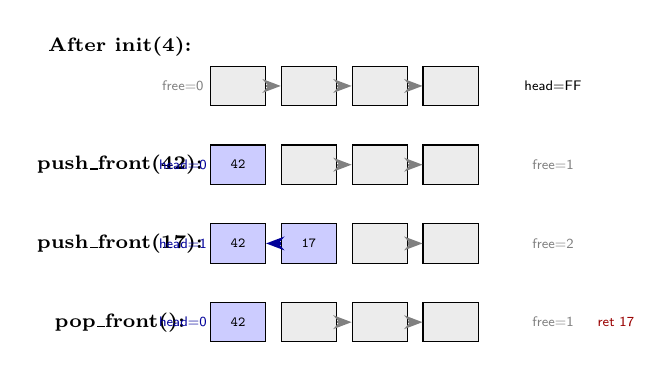
\begin{tikzpicture}[
    >=Stealth,
    cell/.style={draw, minimum width=0.7cm, minimum height=0.5cm,
                 font=\tiny\ttfamily},
    lbl/.style={font=\tiny\sffamily}
  ]
  % Step 1: After init (cap=4)
  \node[font=\scriptsize\bfseries] at (-1.5, 0.5) {After init(4):};
  \foreach \i/\c in {0/gray!15, 1/gray!15, 2/gray!15, 3/gray!15} {
    \node[cell, fill=\c] (a\i) at (\i*0.9, 0) {};
  }
  \node[lbl, text=gray] at (-0.7, 0) {free=0};
  \draw[->, gray, thick] (a0) -- (a1);
  \draw[->, gray, thick] (a1) -- (a2);
  \draw[->, gray, thick] (a2) -- (a3);
  \node[lbl] at (4.0, 0) {head=FF};

  % Step 2: push_front(42)
  \node[font=\scriptsize\bfseries] at (-1.5, -1.0) {push\_front(42):};
  \node[cell, fill=blue!20] (b0) at (0, -1.0) {42};
  \foreach \i/\c in {1/gray!15, 2/gray!15, 3/gray!15} {
    \node[cell, fill=\c] (b\i) at (\i*0.9, -1.0) {};
  }
  \node[lbl, text=blue!60!black] at (-0.7, -1.0) {head=0};
  \draw[->, gray, thick] (b1) -- (b2);
  \draw[->, gray, thick] (b2) -- (b3);
  \node[lbl, text=gray] at (4.0, -1.0) {free=1};

  % Step 3: push_front(17)
  \node[font=\scriptsize\bfseries] at (-1.5, -2.0) {push\_front(17):};
  \node[cell, fill=blue!20] (c0) at (0, -2.0) {42};
  \node[cell, fill=blue!20] (c1) at (0.9, -2.0) {17};
  \foreach \i/\c in {2/gray!15, 3/gray!15} {
    \node[cell, fill=\c] (c\i) at (\i*0.9, -2.0) {};
  }
  \draw[->, blue!60!black, thick] (c1) -- (c0);
  \node[lbl, text=blue!60!black] at (-0.7, -2.0) {head=1};
  \draw[->, gray, thick] (c2) -- (c3);
  \node[lbl, text=gray] at (4.0, -2.0) {free=2};

  % Step 4: pop_front() -> 17
  \node[font=\scriptsize\bfseries] at (-1.5, -3.0) {pop\_front():};
  \node[cell, fill=blue!20] (d0) at (0, -3.0) {42};
  \node[cell, fill=gray!15] (d1) at (0.9, -3.0) {};
  \foreach \i/\c in {2/gray!15, 3/gray!15} {
    \node[cell, fill=\c] (d\i) at (\i*0.9, -3.0) {};
  }
  \node[lbl, text=blue!60!black] at (-0.7, -3.0) {head=0};
  \draw[->, gray, thick] (d1) -- (d2);
  \draw[->, gray, thick] (d2) -- (d3);
  \node[lbl, text=gray] at (4.0, -3.0) {free=1};
  \node[lbl, text=red!60!black] at (4.8, -3.0) {ret 17};
\end{tikzpicture}
\end{center}
\end{frame}

% ===========================================================================
\section{Implementation Details}
% ===========================================================================

\begin{frame}[fragile]{Push Front and Pop Front}
\begin{columns}[T]
\begin{column}{0.48\textwidth}
\begin{lstlisting}[style=cstyle,
  title={push\_front --- $O(1)$}]
int tiku_kits_ds_list_push_front(
    struct tiku_kits_ds_list *list,
    tiku_kits_ds_elem_t value)
{
    uint8_t idx;

    if (list == NULL) {
        return TIKU_KITS_DS_ERR_NULL;
    }

    idx = pool_alloc(list);
    if (idx == TIKU_KITS_DS_LIST_NONE) {
        return TIKU_KITS_DS_ERR_FULL;
    }

    list->pool[idx].data = value;
    list->pool[idx].next = list->head;
    list->head = idx;
    list->count++;
    return TIKU_KITS_DS_OK;
}
\end{lstlisting}
\end{column}

\begin{column}{0.48\textwidth}
\begin{lstlisting}[style=cstyle,
  title={pop\_front --- $O(1)$}]
int tiku_kits_ds_list_pop_front(
    struct tiku_kits_ds_list *list,
    tiku_kits_ds_elem_t *value)
{
    uint8_t idx;

    if (list == NULL || value == NULL) {
        return TIKU_KITS_DS_ERR_NULL;
    }
    if (list->head ==
            TIKU_KITS_DS_LIST_NONE) {
        return TIKU_KITS_DS_ERR_EMPTY;
    }

    idx = list->head;
    *value = list->pool[idx].data;
    list->head = list->pool[idx].next;
    pool_free(list, idx);
    list->count--;
    return TIKU_KITS_DS_OK;
}
\end{lstlisting}
\end{column}
\end{columns}
\end{frame}

% ---------------------------------------------------------------------------
\begin{frame}[fragile]{Traversal with head/next}
\begin{columns}[T]
\begin{column}{0.52\textwidth}
\begin{lstlisting}[style=cstyle,
  title={Iterating through the list}]
struct tiku_kits_ds_list lst;
tiku_kits_ds_elem_t val;
uint8_t cur;

tiku_kits_ds_list_init(&lst, 8);

/* Build list [10, 20, 30, 40] */
tiku_kits_ds_list_push_back(&lst, 10);
tiku_kits_ds_list_push_back(&lst, 20);
tiku_kits_ds_list_push_back(&lst, 30);
tiku_kits_ds_list_push_back(&lst, 40);

/* Traverse using head/next */
cur = tiku_kits_ds_list_head(&lst);
while (cur != TIKU_KITS_DS_LIST_NONE) {
    tiku_kits_ds_list_get(&lst, cur,
                          &val);
    /* process val: 10, 20, 30, 40 */
    cur = tiku_kits_ds_list_next(
              &lst, cur);
}
\end{lstlisting}
\end{column}

\begin{column}{0.44\textwidth}
\begin{center}
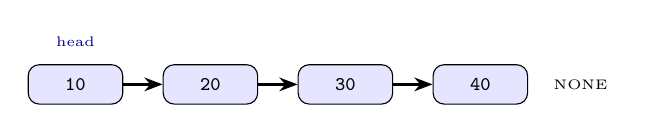
\begin{tikzpicture}[
    >=Stealth,
    node/.style={draw, rounded corners, minimum width=1.2cm,
                 minimum height=0.5cm, font=\scriptsize\ttfamily,
                 fill=blue!10}
  ]
  \node[node] (n0) {10};
  \node[node, right=0.5cm of n0] (n1) {20};
  \node[node, right=0.5cm of n1] (n2) {30};
  \node[node, right=0.5cm of n2] (n3) {40};

  \draw[->, thick] (n0) -- (n1);
  \draw[->, thick] (n1) -- (n2);
  \draw[->, thick] (n2) -- (n3);
  \node[font=\tiny, right=0.2cm of n3] {NONE};
  \node[font=\tiny, above=0.1cm of n0, text=blue!60!black] {head};
\end{tikzpicture}
\end{center}

\vspace{1em}
\begin{block}{Index-Based Iteration}
\begin{itemize}
  \item \texttt{head()} returns pool index of first node
  \item \texttt{next(idx)} returns pool index of successor
  \item \texttt{get(idx, \&val)} reads data at index
  \item \texttt{LIST\_NONE} signals end
\end{itemize}
No pointer dereferencing --- all array indexing.
\end{block}
\end{column}
\end{columns}
\end{frame}

% ===========================================================================
\section{Examples}
% ===========================================================================

\begin{frame}[fragile]{Example 1: Timer List}
\begin{lstlisting}[style=cstyle,
  title={Managing active timers with a linked list}]
struct tiku_kits_ds_list timers;
tiku_kits_ds_elem_t timer_id;
uint8_t idx;

tiku_kits_ds_list_init(&timers, 8);

/* Register timers */
tiku_kits_ds_list_push_back(&timers, TIMER_SENSOR);
tiku_kits_ds_list_push_back(&timers, TIMER_HEARTBEAT);
tiku_kits_ds_list_push_back(&timers, TIMER_DISPLAY);

/* Cancel a specific timer */
if (tiku_kits_ds_list_find(&timers, TIMER_HEARTBEAT, &idx)
    == TIKU_KITS_DS_OK) {
    tiku_kits_ds_list_remove(&timers, idx);
}
/* timers: [TIMER_SENSOR, TIMER_DISPLAY] */

/* Process all remaining timers */
while (tiku_kits_ds_list_pop_front(&timers, &timer_id)
       == TIKU_KITS_DS_OK) {
    fire_timer(timer_id);
}
\end{lstlisting}
\end{frame}

% ---------------------------------------------------------------------------
\begin{frame}[fragile]{Example 2: Sensor Registry}
\begin{columns}[T]
\begin{column}{0.52\textwidth}
\begin{lstlisting}[style=cstyle,
  title={Dynamic sensor registration}]
#define SENSOR_TEMP   1
#define SENSOR_HUMID  2
#define SENSOR_LIGHT  3
#define SENSOR_ACCEL  4

struct tiku_kits_ds_list sensors;
tiku_kits_ds_elem_t sid;
uint8_t cur;

tiku_kits_ds_list_init(&sensors, 8);

/* Register active sensors */
tiku_kits_ds_list_push_back(
    &sensors, SENSOR_TEMP);
tiku_kits_ds_list_push_back(
    &sensors, SENSOR_HUMID);
tiku_kits_ds_list_push_back(
    &sensors, SENSOR_LIGHT);

/* Poll all registered sensors */
cur = tiku_kits_ds_list_head(&sensors);
while (cur !=
       TIKU_KITS_DS_LIST_NONE) {
    tiku_kits_ds_list_get(
        &sensors, cur, &sid);
    read_sensor((uint8_t)sid);
    cur = tiku_kits_ds_list_next(
              &sensors, cur);
}
\end{lstlisting}
\end{column}

\begin{column}{0.44\textwidth}
\begin{center}
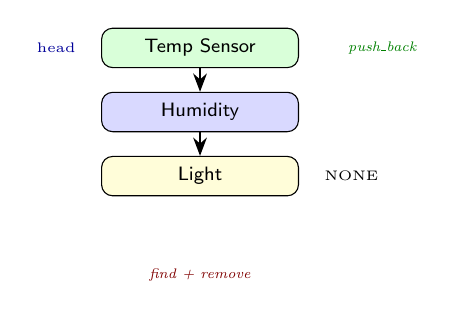
\begin{tikzpicture}[
    >=Stealth,
    box/.style={draw, rounded corners, minimum width=2.5cm,
                minimum height=0.5cm, font=\scriptsize\sffamily}
  ]
  \node[box, fill=green!15] (s1) {Temp Sensor};
  \node[box, fill=blue!15, below=0.3cm of s1] (s2) {Humidity};
  \node[box, fill=yellow!15, below=0.3cm of s2] (s3) {Light};

  \draw[->, thick] (s1) -- (s2);
  \draw[->, thick] (s2) -- (s3);
  \node[font=\tiny, right=0.2cm of s3] {NONE};
  \node[font=\tiny, left=0.2cm of s1, text=blue!60!black] {head};

  % Add/remove annotation
  \node[font=\tiny\itshape, text=green!50!black, right=0.5cm of s1]
    {push\_back};
  \node[font=\tiny\itshape, text=red!50!black, below=0.8cm of s3]
    {find + remove};
\end{tikzpicture}
\end{center}

\vspace{0.5em}
\begin{block}{Dynamic Registration}
Sensors can be added/removed at runtime without
shifting array elements. The pool allocator handles
memory management automatically.
\end{block}
\end{column}
\end{columns}
\end{frame}

% ---------------------------------------------------------------------------
\begin{frame}[fragile]{Example 3: Insert After for Ordered Lists}
\begin{lstlisting}[style=cstyle,
  title={Building an ordered list with insert\_after}]
struct tiku_kits_ds_list lst;
uint8_t head_idx, next_idx;
tiku_kits_ds_elem_t val;

tiku_kits_ds_list_init(&lst, 8);

/* Start with [10, 30] */
tiku_kits_ds_list_push_back(&lst, 10);
tiku_kits_ds_list_push_back(&lst, 30);

/* Insert 20 after head (10) -> [10, 20, 30] */
head_idx = tiku_kits_ds_list_head(&lst);
tiku_kits_ds_list_insert_after(&lst, head_idx, 20);

/* Verify traversal: 10 -> 20 -> 30 */
head_idx = tiku_kits_ds_list_head(&lst);
tiku_kits_ds_list_get(&lst, head_idx, &val);    /* val == 10 */

next_idx = tiku_kits_ds_list_next(&lst, head_idx);
tiku_kits_ds_list_get(&lst, next_idx, &val);    /* val == 20 */

next_idx = tiku_kits_ds_list_next(&lst, next_idx);
tiku_kits_ds_list_get(&lst, next_idx, &val);    /* val == 30 */
\end{lstlisting}
\end{frame}

% ===========================================================================
\section{Test Suite}
% ===========================================================================

\begin{frame}{Test Cases Overview}
\begin{table}
\centering
\small
\begin{tabular}{@{}clp{7cm}@{}}
\toprule
\textbf{\#} & \textbf{Test Function} & \textbf{What It Verifies} \\
\midrule
1 & \texttt{test\_kits\_ds\_list\_init}
  & Initialization, parameter validation \\
2 & \texttt{test\_kits\_ds\_list\_push\_front\_pop}
  & Push front/pop front LIFO order, overflow \\
3 & \texttt{test\_kits\_ds\_list\_push\_back}
  & Push back FIFO order, empty list edge case \\
4 & \texttt{test\_kits\_ds\_list\_insert\_after}
  & Insert after arbitrary node, verify order \\
5 & \texttt{test\_kits\_ds\_list\_remove\_node}
  & Remove head, middle, from empty list \\
6 & \texttt{test\_kits\_ds\_list\_find}
  & Linear search, not-found, empty list \\
7 & \texttt{test\_kits\_ds\_list\_traversal}
  & head/next traversal, single-node list \\
8 & \texttt{test\_kits\_ds\_list\_clear\_reset}
  & Clear rebuilds free pool, list reusable \\
9 & \texttt{test\_kits\_ds\_list\_null\_inputs}
  & All functions reject NULL with ERR\_NULL \\
\bottomrule
\end{tabular}
\end{table}
\end{frame}

% ===========================================================================
\section{Summary}
% ===========================================================================

\begin{frame}{Summary}
\begin{columns}[T]
\begin{column}{0.48\textwidth}
\begin{block}{What We Built}
\begin{itemize}
  \item Pool-allocated singly linked list
  \item Static array with index-based links
  \item Free-list allocator (no heap)
  \item 86 bytes RAM (default 16 nodes), no \texttt{malloc}
  \item $O(1)$ push/pop front, $O(n)$ push back
\end{itemize}
\end{block}

\begin{block}{Key Design Choices}
\begin{itemize}
  \item \texttt{uint8\_t} indices instead of pointers
  \item Free list threaded through pool array
  \item \texttt{LIST\_NONE = 0xFF} sentinel
  \item Active list validation before access
\end{itemize}
\end{block}
\end{column}

\begin{column}{0.48\textwidth}
\begin{block}{Use Cases}
\begin{itemize}
  \item Timer lists with dynamic add/cancel
  \item Task queues with insertion/removal
  \item Sensor/peripheral registry
  \item Event handler chains
\end{itemize}
\end{block}

\begin{block}{Files}
\scriptsize
\begin{tabular}{@{}lp{4.5cm}@{}}
Header: & \texttt{ds/list/tiku\_kits\_ds\_list.h} \\
Source: & \texttt{ds/list/tiku\_kits\_ds\_list.c} \\
Tests: & \texttt{tests/ds/test\_kits\_ds\_list.c} \\
Common: & \texttt{ds/tiku\_kits\_ds.h} \\
\end{tabular}
\end{block}
\end{column}
\end{columns}
\end{frame}

% ---------------------------------------------------------------------------
\begin{frame}{Thank You}
\begin{center}
\Large\textbf{TikuKits DS: Linked List}\\[0.5em]
\normalsize Pool-Allocated Data Structures for Physical AI Endpoints\\[1.5em]

\begin{tabular}{rl}
  Repository: & \url{https://github.com/tikuos/tikuOS} \\
  License:    & Apache 2.0 \\
  Common:     & \texttt{tikukits/ds/tiku\_kits\_ds.h} \\
  Header:     & \texttt{tikukits/ds/list/tiku\_kits\_ds\_list.h} \\
  Source:     & \texttt{tikukits/ds/list/tiku\_kits\_ds\_list.c} \\
  Tests:      & \texttt{tikukits/tests/ds/test\_kits\_ds\_list.c} \\
\end{tabular}
\end{center}
\end{frame}

\end{document}
